%!TEX root = sbgames-metalearning.tex
\section{Experiments and Results}
\label{sec:results}

In this section, we detail our implementation of meta-level reinforcement learning and its integration to the \emph{Starcraft} game, followed by our experiments and their results. 



\subsection{Interacting with StarCraft}
\label{subsec:bwapi}

The first challenge in implementing the algorithm is the integration of our learning algorithm to the proprietary code from Starcraft, since we cannot directly modify its code and need external tools to do this. 
In the case of StarCraft, community members developed the \textit{BWAPI}, which allows us to inject code into the existing game binaries. 
The \textit{BWAPI (Brood War Application Programming Interface)}\footnote{An API to interact with StarCraft: BroodWar \url{http://code.google.com/p/bwapi/}} enables the creation and injection of artificial intelligence code into StarCraft. 
BWAPI was initially developed in \textit{C++}, and later ported to other languages like \textit{Java}, \textit{C\#} and \textit{Python}, and divides StarCraft in 4 basic types of object:


\begin{itemize}
\item \textit{Game:} manages information about the current game being played, 
including the position of known units, location of resources, etc.;
\item \textit{Player:} manages the information available to a player, such as: 
available resources, buildings and controllable units;
\item \textit{Unit:} represents a piece in the game, either mineral, construction or combat unit;
\item \textit{Bullet:} represents a projectile fired from a ranged unit;
\end{itemize}

Since the emergence of BWAPI in 2009, StarCraft has drawn the attention of researchers and an active community of bot programming has emerged~\cite{buro2012real}. 
For our implementation, we modified the open source bot \textit{BTHAI}~\cite{hagelback2012potential},
adding a high-level strategy learning component to it\footnote{The source code can be fount at: \url{https://github.com/jieverson/BTHAIMOD}}.
Figure~\ref{fig:game-play} shows a screenshot of a game where one of the players is controlled by BTHAI, notice the additional information overlaid on the game interface. 

\begin{figure}[ht]
\centering
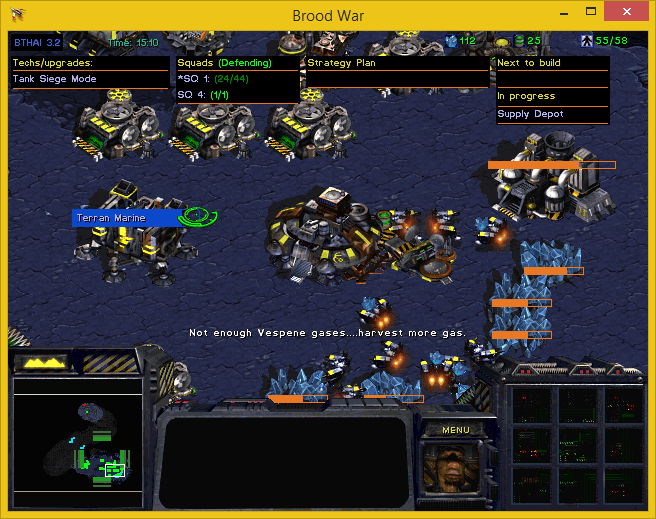
\includegraphics[width=250px]{images/game-play}
\caption{BTHAI bot playing StarCraft: Brood War.}
\label{fig:game-play}
\end{figure}



\subsection{A Reinforcement Learning Approach for StarCraft}
\label{subsec:rl-sc}

Following the approach used by~\cite{amato2010highlevel}, our approach focuses on learning the best high-level strategy to use against an opponent. 
We assume here that the agent will only play as Terran, and will be able to choose any one of the following strategies:

\begin{itemize}
\item \textit{Marine Rush:} is a very simple Terran strategy that relies on quickly creating a specific number of workers (just enough to maintain the army) and then spending all the acquired resources on the creation of Marines (the cheapest Terran battle unit) and making an early attack with a large amount of units.

\item \textit{Wraith Harass:} is similar, but slightly improved, Marine rush that consists of adding 
a mixture of 2--5 Wraiths (a relatively expensive flying unit) to the group of Marines. The Wraith's mission is to attack the opponent from a safe distance, and when any of the Wraiths are in danger,  use some Marines to protect it.
Unlike the Marine Rush, this strategy requires strong micromanagement, making it more difficult to perform. 

\item \textit{Terran Defensive:} consists of playing defensively and waiting for the opponent to attack before counterattacking. 
Combat units used in this strategy are Marines and Medics (a support unit that can heal biological units),
usually defended by a rearguard of Siege Tanks.

\item \textit{Terran Defensive FB:} is slightly modified version of the Terran Defensive strategy, which replaces up to half of the Marines by Firebats --- a unit equipped with flamethrowers that is 
especially strong against non-organic units such as aircrafts, tanks and most of Protoss' units.

\item \textit{Terran Push:} consists of creating approximately five Siege Tanks and a large group of Marines, and moving these units together through the map in stages, stopping at regular intervals to regroup. 
Given the long range of the Tank's weapons, opponents will often not perceive their approach until their units are under fire, however, this setup is vulnerable to air counterattack units. 
\end{itemize}

After each game, the agent observes the end result (victory or defeat), and uses this feedback to learn the best strategy. 
If the game is played again, the learning continues, so we can choose the strategy with the highest value for the current situation. 
If the agent perceives, at any time, that the strategy ceases to be effective 
--- because of a change in the opponent's strategy, map type, race or other factors ---
the agent is able to quickly readapt to the new conditions, choosing a new strategy.



\subsection{Experiments with StarCraft}
\label{subsec:experiments}

To demonstrate the applicability of our approach we have designed an experiment whereby a number of games are played against a single opponent that can play using different AI bot strategies. 
We seek to determine if our learning methods can adapt its policy when the AI bot changes. 
Each game was played in a small two-player map (\textit{Fading Realm}) using the maximum game speed (since all players were automated).
The game was configured to start another match as soon as the current one ends.
For the experiment, all the Q-values are initialized to $0$, and the learning-rate ($\alpha$) is initialized to $0.5$. 
Our experiment consisted of playing the game a total of 138 matches where one of the players is controlled by an implementation of our meta-learning agent. 
In the first $55$ matches, the opponent have played a fixed Terrain policy provided by the game and in subsequent matches, we have changed the opponent policy to the fixed Protoss policy provided by the game. 
It is worth noting that our method used very little computation time--it runs in real time, using accelerated game speed (for matches between two bots).

\begin{figure}[ht]
\centering
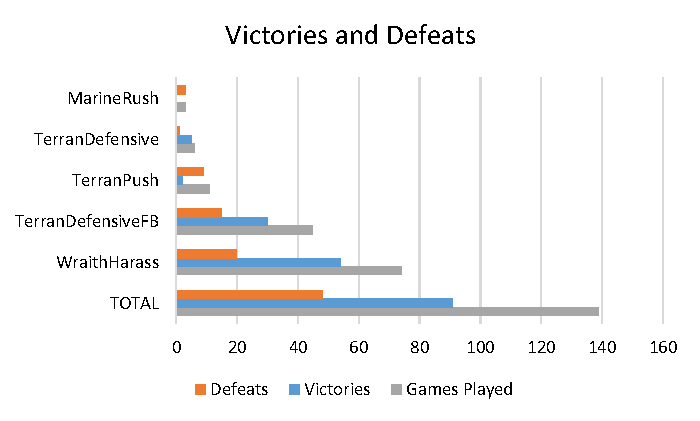
\includegraphics[width=250px]{images/wins_graphic}
\caption{Comparison between the number of victories and defeats of each strategy.}
\label{fig:wins_graphic}
\end{figure}

\begin{figure}[ht]
\centering
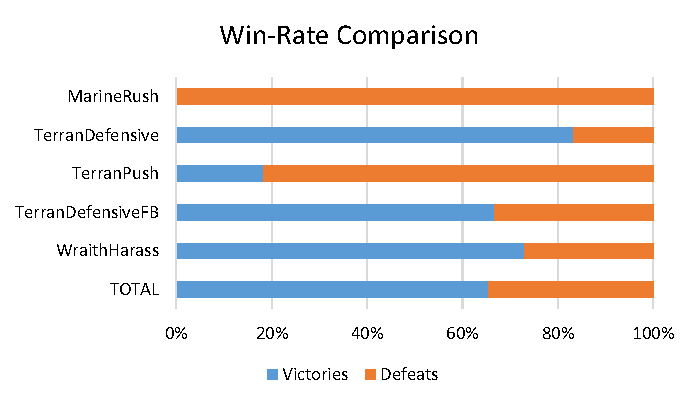
\includegraphics[width=250px]{images/win-rates_graphic}
\caption{Graphic that presents a comparation between the win rate of each strategy.}
\label{fig:win-rates_graphic}
\end{figure}

The results obtained are illustrated in the graph of Figure~\ref{fig:wins_graphic} and Figure~\ref{fig:win-rates_graphic}, which shows that our meta-learning agent consistently outperforms fixed opponents. 
Moreover, we can see that the agent quickly learns the best strategy to win against a fixed policy opponent when its strategy changes. 
As it learns, its learning-rate should tend to decrease towards $0$, which means that the agent has nothing to learn.
After the change in opponent policy (at game execution $55$), we expected the learning-rate to   increase, denoting that the agent is starting to learn again, which was indeed the case, as illustrated by the graph of Figure~\ref{fig:learning-rate_graphic}. 
The learning rate should remain above $0$ until the RL algorithm converges to the optimal policy, and then start decreasing towards $0$.
We note that, although the learning-rate may vary between $0$ and $1$, it has never gone beyond $0.7$ in the executions we performed.

\begin{figure}[ht]
\centering
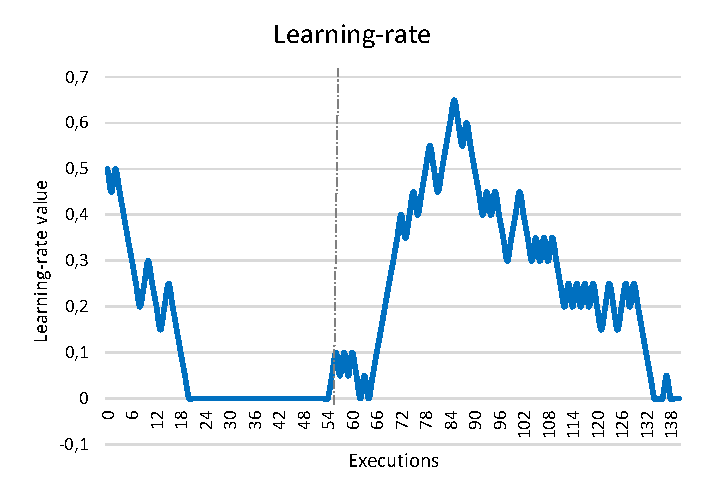
\includegraphics[width=250px]{images/learning-rate_graphic}
\caption{Learning-rate variation over time.}
\label{fig:learning-rate_graphic}
\end{figure}

Finally, the graphic in Figure~\ref{fig:strategies_graphic} illustrates the variation
of the strategies Q-values over each game execution.
We can see that the \textit{Wraith Harass} strategy was optimal against the first opponent policy, 
while the \textit{Terrain Push} has proven to be the worst.
When the opponent changes its policy, we can see the Q-value of \textit{Wraith Harass} decreases,
resulting in an increase in exploration. 
After the execution $85$, we notice that the \textit{Terrain Defensive FB} strategy stood out from the others, although the basic \textit{Terrain Defensive} strategy has shown to yield good results too. 
\textit{Wraith Harass} and \textit{Marine Rush} seem to lose to the second opponent policy, 
and \textit{Terrain Push} shows remain the worst strategy. 

\begin{figure}[ht]
\centering
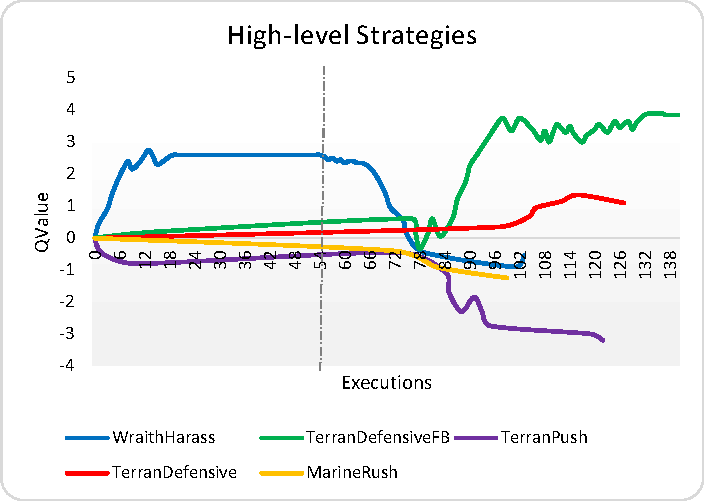
\includegraphics[width=250px]{images/strategies_graphic}
\caption{Strategies Q-Value over time.}
\label{fig:strategies_graphic}
\end{figure}